\documentclass[tikz,border=8pt]{standalone}
% Shared look for every TikZ diagram. Load with \input{../../tools/tikz-style.tex}
\usepackage[T1]{fontenc}
\usepackage{lmodern}
\renewcommand{\sfdefault}{lmr}  % diagrams use the same serif as the text
\usetikzlibrary{arrows.meta, positioning, shapes.geometric, calc, fit, backgrounds}
\definecolor{cblue}{HTML}{4C78A8}
\definecolor{corange}{HTML}{F58518}
\definecolor{cgreen}{HTML}{54A24B}
\definecolor{cred}{HTML}{E45756}
\definecolor{cpurple}{HTML}{B279A2}
\definecolor{cgrey}{HTML}{6B6B6B}
\tikzset{
  every picture/.style={font=\sffamily, line width=1.2pt},
  box/.style={draw=#1, fill=#1!12, rounded corners=4pt, align=center, inner sep=7pt, minimum height=1.1cm},
  box/.default=cgrey,
  arrow/.style={-{Stealth[length=3mm]}, draw=cgrey, line width=1.4pt},
  title/.style={font=\sffamily\bfseries\Large},
  note/.style={font=\sffamily\small, text=cgrey, align=center},
}
\AtBeginDocument{\hyphenpenalty=10000 \exhyphenpenalty=10000}

\begin{document}
% Section 3: the plain encoder-decoder hands the same context vector to every decoder step.
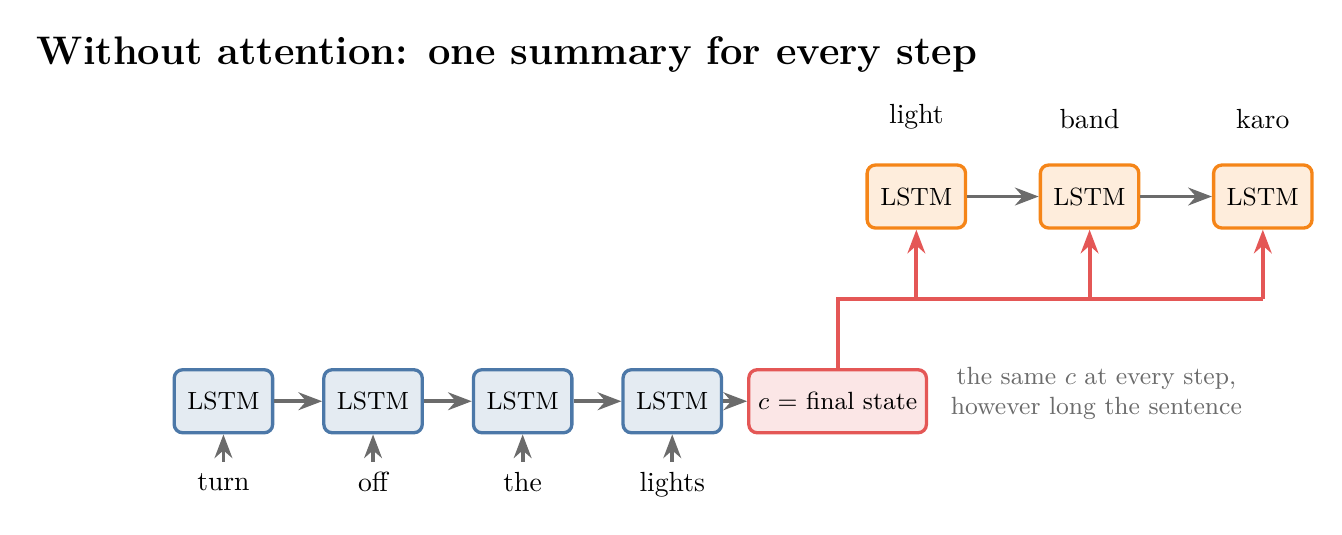
\begin{tikzpicture}[cell/.style={draw=#1, fill=#1!15, minimum width=1.25cm, minimum height=0.8cm, rounded corners=3pt, font=\sffamily\small},
  word/.style={font=\sffamily}]
  \node[title] at (5.5, 4.4) {Without attention: one summary for every step};
  \foreach \w [count=\j] in {turn, off, the, lights} {
    \node[cell=cblue] (e\j) at (1.9*\j, 0) {LSTM};
    \node[word, below=0.35cm of e\j] (x\j) {\w};
    \draw[arrow] (x\j) -- (e\j);
  }
  \foreach \i/\j in {1/2, 2/3, 3/4} \draw[arrow] (e\i) -- (e\j);
  \node[draw=cred, fill=cred!15, rounded corners=3pt, minimum height=0.8cm, font=\sffamily\small] (c) at (9.7, 0) {$c$ = final state};
  \draw[arrow] (e4) -- (c);
  \foreach \w [count=\i] in {light, band, karo} {
    \node[cell=corange] (d\i) at (8.5 + 2.2*\i, 2.6) {LSTM};
    \node[word, above=0.3cm of d\i] {\w};
    \draw[arrow, draw=cred] (8.5 + 2.2*\i, 1.3) -- (d\i.south);
  }
  \draw[draw=cred, line width=1.4pt] (c.north) |- (15.1, 1.3);
  \draw[arrow] (d1) -- (d2); \draw[arrow] (d2) -- (d3);
  \node[note, anchor=west] at (11.0, 0.1) {the same $c$ at every step,\\however long the sentence};
\end{tikzpicture}
\end{document}
